\chapter{분포 모형화 (Modeling distributions)}
\label{modeling}

지금까지 사용한 분포는 {\bf 경험적 분포 (empirical distributions)}라고 부른다.
이유는 필연적으로 유한 표본인 경험적 관측치에 기반하고 있기 때문이다.

\index{해석 분포 (analytic distribution)}
\index{분포 (distribution)!해석 (analytic)}
\index{경험적 분포 (empirical distribution)}
\index{분포 (distribution)!경험 (empirical)}

수학 함수인 CDF로 특징 지어지는 {\bf 해석 분포 (analytic distribution)}가 대안이 된다.
해석 분포가 경험적 분포를 모형화하는데 사용될 수 있다.
이러한 맥락에서 {\bf 모형(model)}은 불필요한 부분을 덜어낸 단순화가 된다.
이번 장에서 자주 사용되는 분포를 제시하고 이를 사용하여 다양한 출처를 가진 
데이터를 모형화한다.

\index{모형 (model)}

이번 장에서 사용되는 코드는 {\tt analytic.py}에 있다.
코드를 다운로드하고 작업하는 것에 대한 정보는 ~\ref{code}을 참조한다.


\section{지수분포 (exponential distribution)}
\label{exponential}
\index{지수분포 (exponential distribution)}
\index{분포 (distribution)!지수 (exponential)}

\begin{figure}
% analytic.py
%\centerline{\includegraphics[height=2.5in]{figs/analytic_expo_cdf.pdf}}
\caption{CDFs of exponential distributions with various parameters.}
\label{analytic_expo_cdf}
\end{figure}

{\bf 지수 분포 (exponential distribution)}로 시작하는데 이유는 상대적으로 단순하기 때문이다.
지수분포 CDF는 다음과 같다.
%
\[ \CDF(x) = 1 - e^{-\lambda x} \]
%

모수 $\lambda$가 분포 형상(shape)을 결정한다. 
그림~\ref{analytic_expo_cdf}에서 $\lambda = $ 0.5, 1, 2 값을 가진
CDF가 대략 모양이 어떤지 볼 수 있다.
\index{모수 (parameter)}

현실 세계에서 일련의 사건을 보고, 사건 간에 시간({\bf 도착간격 시간, interarrival times})을 측정할 때 지수분포가 등장한다.
만약 사건이 언제든지 균등하게 발생할 것 같다면 도착간격 시간 분포는 지수분포같은 경향이 있다.
\index{도착간격 시간 (interarrival time)}

일례로, 출생간 발생시간을 살펴보자. 1997년 12월 18일 호주 브리즈번
\footnote{예제에 나오는 자료와 정보는 저널 논문에 기반한다. Dunn, ``A Simple Dataset for Demonstrating Common Distributions,'' Journal of Statistics Education v.7, n.3 (1999)}
에서 44명 신생아가 출생했다. 모든 44명 신생아 출생 시간이 지역신문에 출간되었다;
전체 데이터셋은 {\tt ThinkStats2} 저장소 {\tt babyboom.dat} 파일에 담겨있다.
\index{출생 시간 (birth time)}
\index{호주 (Australia)} 
\index{브리즈번 (Brisbane)}

\begin{verbatim}
    df = ReadBabyBoom()
    diffs = df.minutes.diff()
    cdf = thinkstats2.Cdf(diffs, label='actual')

    thinkplot.Cdf(cdf)
    thinkplot.Show(xlabel='minutes', ylabel='CDF')
\end{verbatim}

{\tt ReadBabyBoom} 함수가 데이터 파일을 읽어들이고 {\tt time}, {\tt sex}, \verb"weight_g", {\tt minutes}
칼럼으로 구성된 데이터프레임을 반환한다.
여기서 {\tt minutes}가 자정 이후 출생시간을 분으로 변환한 시간정보를 담고 있다.
\index{데이터프레임 (DataFrame)}
\index{thinkplot}

\begin{figure}
% analytic.py
%\centerline{\includegraphics[height=2.5in]{figs/analytic_interarrivals.pdf}}
\caption{CDF of interarrival times (left) and CCDF on a log-y scale (right).}
\label{analytic_interarrival_cdf}
\end{figure}

%\begin{figure}
% analytic.py
%%\centerline{\includegraphics[height=2.5in]{figs/analytic_interarrivals_logy.pdf}}
%\caption{CCDF of interarrival times.}
%\label{analytic_interarrival_ccdf}
%\end{figure}

{\tt diffs}는 연속되는 출생시간 사이 차이가 되고 
{\tt cdf}는 출생간격 시간 분포가 된다.
그림~\ref{analytic_interarrival_cdf} (왼편)이 CDF를 나타낸다.
전형적인 지수분포 형상을 지닌 처럼 보이지만, 어떻게 분간할 수 있을까?

한 방법은 {\bf 보완 CDF (complementary CDF)}를 플롯으로 그리는 것이다.
보완 CDF는 log-y 척도로 $1 - \CDF(x)$이다.
지수분포 데이터에 대해서는 결과가 직선이다. 왜 그런지 살펴보자.

\index{보완 CDF (complementary CDF)} 
\index{CDF!보완 (complementary)} 
\index{CCDF}

독자가 생각하기에 지수분포를 따르는 데이터셋을 보완 CDF(CCDF) 플롯으로 그리면, 
다음과 같은 함수가 나올 것으로 기대한다.
%
\[ y \approx e^{-\lambda x} \]
%
양변에 로그를 취하면 다음과 같다.
%
\[ \log y \approx -\lambda x\]
%
그래서, log-y 척도로 CCDF는 기울기 $-\lambda$인 직선이 된다.
다음에 플롯을 생성하는 방법이 있다.
\index{로그 척도 (logarithmic scale)}
\index{보완 CDF (complementary CDF)}
\index{CDF!보완 (complementary)}
\index{CCDF}

\begin{verbatim}
    thinkplot.Cdf(cdf, complement=True)
    thinkplot.Show(xlabel='minutes',
                   ylabel='CCDF',
                   yscale='log')
\end{verbatim}

{\tt complement=True} 인자가 있어서, {\tt thinkplot.Cdf}이 플롯을 그리기 전에
보완 CDF를 계산한다. 그리고 {\tt yscale='log'}를 통해서  
{\tt thinkplot.Show}가 로그 척도로 {\tt y}축을 고정한다.
\index{thinkplot}
\index{Cdf}

그림~\ref{analytic_interarrival_cdf} (오른편)에 결과가 있다.
정확하게 직선이 아니다. 이 데이터에 대해서 완벽한 모델로 지수 분포가 아니라는 것이 표시된다.
기본 가정---출생이 아무 때고 균등하게 발생---이 정확하게 사실이 아닐 것이다.
그럼에도 불구하고 지수분포로 이 데이터셋을 모형화하는 것이 합리적일 것이다.
이와 같은 단순화로 단 하나의 모수로 분포를 요약할 수 있다.
\index{모형 (model)}

모수 $\lambda$가 율(rate)로 해석될 수 있다; 즉, 평균적으로 단위 시간에 
발생하는 사건 수. 예제에서 44명의 신생아가 24시간내에 태어난다.
그래서 율값이 분당 $\lambda = 0.0306$이 된다.
지수분포 평균은 $1/\lambda$ 으로 신생아 간에 출생 평균 시간은 32.7분이 된다.

\section{정규 분포 (normal distribution)}
\label{normal}

가우스 분포(Gaussian distribution)라고도 불리는 
{\bf 정규 분포 (normal distribution)}가 흔히 사용되는데 이유는 많은 현상을 기술하고 
최소한 근사적으로도 기술할 수 있기 때문이다.
\ref{CLT} 절에서 다루게 되는데 이와 같은 보편성에는 이유가 있다.
\index{CDF}
\index{모수 (parameter)}
\index{평균 (mean)}
\index{표준편차 (standard deviation)}
\index{정규 분포 (normal distribution)}
\index{분포 (distribution)!정규 (normal)}
\index{가우스 분포 (Gaussian distribution)}
\index{분포 (distribution)!가우스 (Gaussian)}

%
\[ \CDF(z) = \frac{1}{\sqrt{2 \pi}} \int_{-\infty}^z e^{-t^2/2} dt \]
%

\begin{figure}
% analytic.py
%\centerline{\includegraphics[height=2.5in]{figs/analytic_gaussian_cdf.pdf}}
\caption{CDF of normal distributions with a range of parameters.}
\label{analytic_gaussian_cdf}
\end{figure}

정규 분포는 모수 두개로 특성화된다: 평균 $\mu$, 표준편차 $\sigma$.
모수 $\mu=0$과 $\sigma=1$을 갖는 정규분포를 {\bf 표준 정규 분포 (standard normal
 distribution)}라고 한다.
정규분포 CDF는 닫힌 형식 해법(closed form solution)을 갖지 않는 적분으로 정의된다.
하지만, 효율적으로 계산하는 알고리즘이 있다.
알고리즘 중 하나가 SciPy을 통해 제공된다: {\tt scipy.stats.norm}이
정규분포를 표현하는 객체다. 표준 정규분포 CDF를 계산하는 {\tt cdf} 메쏘드를 제공한다.

\index{SciPy}
\index{닫힌 형식 (closed form)}

\begin{verbatim}
>>> import scipy.stats
>>> scipy.stats.norm.cdf(0)
0.5
\end{verbatim}

결과값은 맞다: 표준 정규분포 중위수는 0 (평균과 같다)이고, 값의 절반이 중위수 아래 위치한다.
그래서 $\CDF(0)$은 0.5 이다.

{\tt norm.cdf}은 옵션 모수를 받는다: {\tt loc}가
평균을 특정하고, {\tt scale}는 표준편차를 특정한다.


{\tt thinkstats2}는 상기 함수를 좀더 사용하기 쉽게 한다.
{\tt EvalNormalCdf} 메쏘드는 {\tt mu}과 {\tt sigma}을 인자로 받아 
{\tt x}에 CDF를 계산한다.

\index{정규 분포 (normal distribution)}

\begin{verbatim}
def EvalNormalCdf(x, mu=0, sigma=1):
    return scipy.stats.norm.cdf(x, loc=mu, scale=sigma)
\end{verbatim}

그림~\ref{analytic_gaussian_cdf}에 정규분포에 다양한 모수를 넣어 그린 CDF가 있다.
곡선의 S자(sigmoid) 형상이 정규분포를 식별할 수 있게 하는 특성이다.

앞장에서 NSFG 출생 체중 분포를 살펴봤다.
모든 정상 출산 체중에 대한 경험적 CDF와 동일한 평균과 분산으로 정규분포 CDF를 중첩하여 
플롯으로 그린 것이 그림~\ref{analytic_birthwgt_model}이다.

\index{가족 성장 국가 조사 (National Survey of Family Growth)}
\index{NSFG}
\index{출생 체중 (birth weight)}
\index{체중 (weight)!출생 (birth)}

\begin{figure}
% analytic.py
%\centerline{\includegraphics[height=2.5in]{figs/analytic_birthwgt_model.pdf}}
\caption{CDF of birth weights with a normal model.}
\label{analytic_birthwgt_model}
\end{figure}

정규분포가 이 데이터셋에 대해서 좋은 모형이 된다.
그래서 만약 모수 $\mu = 7.28$과 $\sigma = 1.24$으로 
분포를 요약한다면, 결과 오차(모형과 데이터 간 차이)가 작다.

\index{모형 (model)}
\index{백분위수 (percentile)}

백분위수 10번째 아래에서 데이터와 모형 사이에 불일치가 있다.
정규분포에서 예측되는 것보다 더 많이 체중이 적은 아이가 있다.
만약 조산아에 특별히 관심이 있다면, 분포에서 이 부분을 잘 적합하는 것이 중요하다.
그래서 정규분포를 사용하는 것이 적절하지 않을 수도 있다.


\section{정규확률그림 (Normal probability plot)}

지수분포와 몇가지 분포에서 대해서 해석분포(analytic distribution)가 특정 데이터셋에 대해서
적합한 모형인가를 테스트하는데 사용할 수 있는 간단한 변환이 있다.

\index{지수분포 (exponential distribution)}
\index{분포 (distribution)!지수 (exponential)}
\index{모형 (model)}

정규분포에 대해서 그러한 변환은 없다. 하지만, 
{\bf 정규확률그림 (normal probability plot)}으로 불리는 대안이 있다.
정규확률그림을 생성하는 방식이 두개 있다.: 어려운 방식과 쉬운 방식.
어려운 방식에 관심이 있다면 \url{https://en.wikipedia.org/wiki/Normal_probability_plot}에서 
자세한 정보를 얻을 수 있다.
다음에 쉬운 방식이 있다.
\index{정규확률그림 (normal probability plot)}
\index{그림 (plot)! 정규확률 (normal probability)}
\index{정규분포 (normal distribution)}
\index{분포 (distribution)!정규 (normal)}
\index{가우스 분포 (Gaussian distribution)}
\index{분포 (distribution)!가우스 (Gaussian)}

\begin{enumerate}

\item 표본에 있는 값을 정렬한다.

\item 표준정규분포($\mu=0$, $\sigma=1$)에서 표본과 동일한 크기를 갖는 난수을 생성하고
정렬한다.
\index{난수 (random number)}

\item 표본에서 나온 정렬된 값과 난수를 플롯으로 그린다.

\end{enumerate}

만약 표본 분포가 근사적으로 정규분포라면, 결과는 
절편 {\tt mu}, 기울기 {\tt sigma}를 갖는 직선이다.
{\tt thinkstats2}에 {\tt NormalProbability}이 있다.
표본을 인자로 받아서 넘파이(NumPy) 배열 두개를 반환한다.
\index{넘파이 (NumPy)}

\begin{verbatim}
xs, ys = thinkstats2.NormalProbability(sample)
\end{verbatim}

\begin{figure}
% analytic.py
%\centerline{\includegraphics[height=2.5in]{figs/analytic_normal_prob_example.pdf}}
\caption{Normal probability plot for random samples from normal distributions.}
\label{analytic_normal_prob_example}
\end{figure}

{\tt ys}는 {\tt sample}에서 정렬된 값이 담겨있다; 
{\tt xs}에는 표준정규분포에서 생성된 난수가 담겨있다.

{\tt NormalProbability}을 테스트하기 위해서 다양한 모수를 가진 
정규분포에서 모조 샘플을 생성했다.
그림~\ref{analytic_normal_prob_example}에 결과가 있다.
선들이 근사적으로 직선으로, 평균에 있는 값보다 벗어난 값을 꼬리에 갖는다.

이제 실제 데이터에 적합을 시도해 보자.
앞절로부터 출생 체중 데이터에 대해 정규확률그림을 생성하는 코드가 다음에 있다.
모형을 표현하는 회색선과 실제 데이터를 표현하는 파란선을 플롯으로 그린다.

\index{출생 체중 (birth weight)}
\index{체중 (weight)!출생 (birth)}

\begin{verbatim}
def MakeNormalPlot(weights):
    mean = weights.mean()
    std = weights.std()

    xs = [-4, 4]
    fxs, fys = thinkstats2.FitLine(xs, inter=mean, slope=std)
    thinkplot.Plot(fxs, fys, color='gray', label='model')

    xs, ys = thinkstats2.NormalProbability(weights)
    thinkplot.Plot(xs, ys, label='birth weights')
\end{verbatim}

{\tt weights}는 출생 체중 판다스 시리즈다; {\tt mean}과 {\tt std}은
각각 평균과 표준편차다.
\index{판다스 (pandas)}
\index{시리즈 (Series)}
\index{thinkplot}
\index{표준편차 (standard deviation)}

{\tt FitLine}이 시퀀스 {\tt xs}, 절편, 기울기를 인자로 받는다;
반환하는 {\tt xs}와 {\tt ys}는 {\tt xs} 값에서 계산되어 인자로 받은 모수를 가진 직선이다.

{\tt NormalProbability}은 {\tt xs}와 {\tt ys}를 반환하는데 
표준정규분포에서 나온 값과 {\tt weights}에서 나온 값을 담고 있다.
만약 체중 분포가 정규분포를 따른다면, 데이터도 모델과 매칭되어야 한다.

\index{모형 (model)}

\begin{figure}
% analytic.py
%\centerline{\includegraphics[height=2.5in]{figs/analytic_birthwgt_normal.pdf}}
\caption{Normal probability plot of birth weights.}
\label{analytic_birthwgt_normal}
\end{figure}

그림~\ref{analytic_birthwgt_normal}이 전체 정상 출생과 더불어 만삭(임신기간이 36주 이상)에 대한 결과를 보여준다.
두 곡선 모두 평균 근처에서 모형과 매칭되고 꼬리에서 차이가 난다.
가장 무거운 아이가 모형이 예측한 것보다 더 무겁고, 가장 가벼운 아이는 더 가볍다.

\index{임신 기간}

단지 만삭 아이만 선택해서, 가장 가벼운 몇몇 아이를 제거하면 분포 아래쪽 꼬리에 있는 불일치를 줄일 수 있다.

정규분포 모형이 평균에서부터 몇 표준편차 내에서 분포를 잘 기술하지만, 꼬리 부근에서는 아니라고 플롯 그래프를 통해서 알 수 있다.
실제 목적에 얼마나 부합되는지는 목적에 달려있다.
\index{모형 (model)}
\index{출생 체중 (birth weight)}
\index{체중 (weight)!출생 (birth)}
\index{표준편차 (standard deviation)}


\section{로그 정규분포 (lognormal distribution)}
\label{brfss}
\label{lognormal}

만약 값을 로그 취한 집합이 정규분포라면, 이 값은 {\bf 로그 정규분포 (lognormal distribution)}다. 로그 정규분포 CDF는 $x$를 $\log x$로 치환한 정규분포 CDF와 동일하다.
%
\[ CDF_{lognormal}(x) = CDF_{normal}(\log x)\]
%
로그 정규분포 모수는 일반적으로 $\mu$와 $\sigma$로 표기한다.
하지만, 기억할 것은 모수가 평균과 표준편차는 {\em 아니다};
로그 정규분포 평균은 $\exp(\mu +\sigma^2/2)$이고, 표준편차는 조금 복잡한다.(\url{http://wikipedia.org/wiki/Log-normal_distribution}를 참조한다)
\index{모수 (parameter)} 
\index{체중 (weight)!성인 (adult)} 
\index{성인 체중 (adult weight)}
\index{로그 정규분포 (lognormal distribution)}
\index{분포 (distribution)!로그 정규 (lognormal)}
\index{CDF}

\begin{figure}
% brfss.py
%\centerline{
%\includegraphics[height=2.5in]{figs/brfss_weight.pdf}}
%\caption{CDF of adult weights on a linear scale (left) and
%log scale (right).}
%\label{brfss_weight}
\end{figure}

만약 표본이 근사적으로 로그 정규분포이고 log-x 척도로 CDF 플롯을 그린다면, 정규분포 특성의 형상을 갖는다.
표본이 로그 정규분포 모형과 얼마나 잘 적합하는지 테스트하기 위해서, 
표본값에 로그를 취해서 정규확률그림을 생성할 수 있다.

\index{정규확률그림 (normal probability plot)}
\index{모형 (model)}

예제로 성인 체중 분포를 살펴보는데 근사적으로 로그 정규분포다.\footnote{\url{http://mathworld.wolfram.com/LogNormalDistribution.html} 사이트에서 주석(인용없이)으로 이 가능성에 대해서 제보를 받았다.
나중에 로그 변환과 원인을 제안하는 논문을 발견했다: Penman and Johnson, ``The Changing Shape of the Body Mass Index Distribution Curve in the Population,'' Preventing Chronic Disease, 2006 July; 3(3): A74.  Online at \url{http://www.ncbi.nlm.nih.gov/pmc/articles/PMC1636707}.}


만성 질환 예방 및 건강 증진을 위한 국립 센터 (National Center for Chronic Disease Prevention and Health Promotion)에서는 
행동 위험 요인 감시 시스템(Behavioral Risk Factor Surveillance System, BRFSS)\footnote{질병통제 예방센터(Centers for Disease Control and Prevention, CDC). 행동 위험 요인 감시 시스템 조사 자료(Behavioral Risk Factor Surveillance System Survey Data). Atlanta, Georgia: 미국 보건 복지부 (U.S. Department of Health and Human Services), 질병통제 예방센터 (Centers for Disease Control and Prevention), 2008.}의 일부문으로 매년 조사를 실시한다.
2008년 414,509 응답자를 대상으로 인터뷰했고 인구통계, 건강, 건강 위험에 관해서 설문했다. 수집한 데이터 중에 398,484 응답자 킬로그램으로 표시된 체중정보가 있다.
\index{행동 위험 요인 감시 시스템 (Behavioral Risk Factor Surveillance System)}
\index{BRFSS}

이 책을 위한 저장소에 BRFSS에 관한 데이터를 담고 있는 고정폭 아스키(ASCII)파일, {\tt CDBRFS08.ASC.gz}와 더불어 파일을 읽고 데이터를 분석하는 {\tt brfss.py}파일도 함께 있다.

\begin{figure}
% brfss.py
%\centerline{
%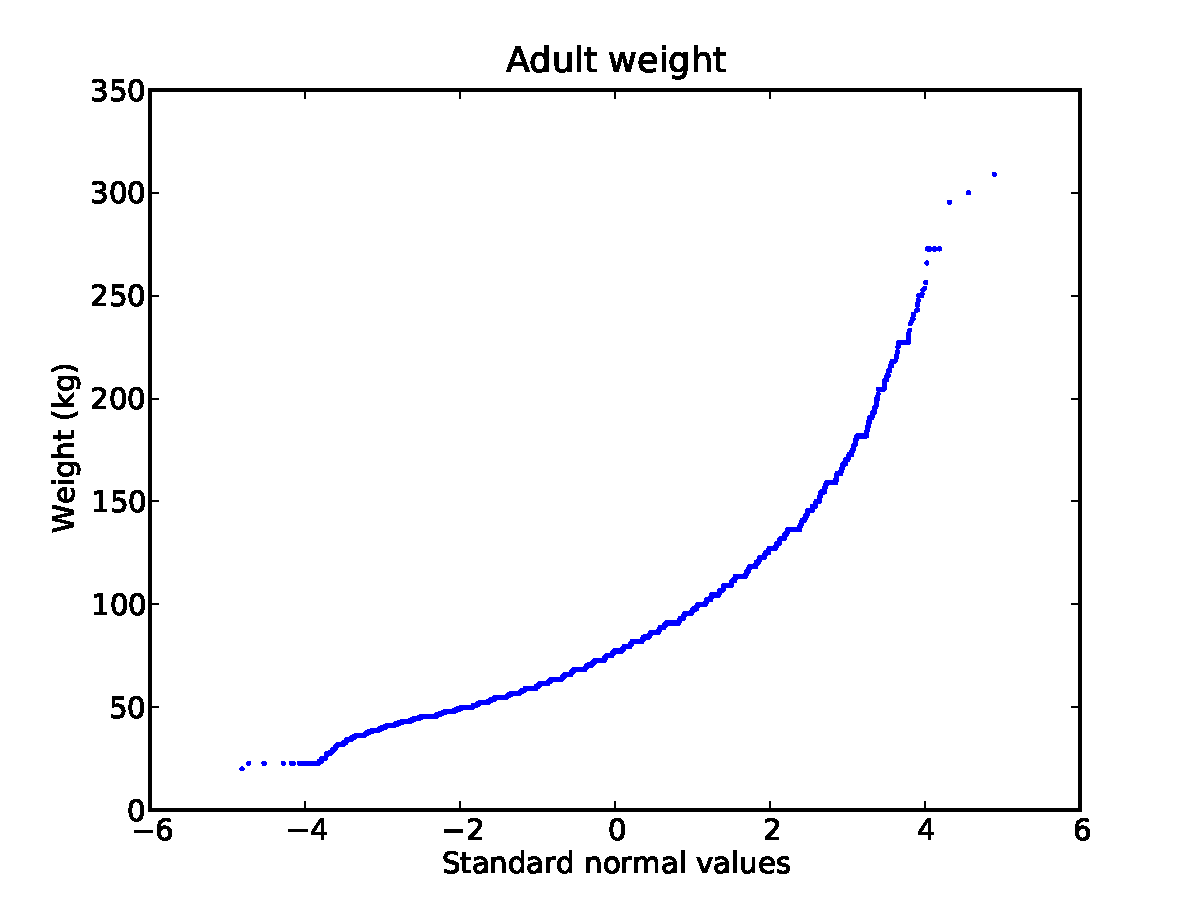
\includegraphics[height=2.5in]{figs/brfss_weight_normal.pdf}}
\caption{Normal probability plots for adult weight on a linear scale
  (left) and log scale (right).}
\label{brfss_weight_normal}
\end{figure}

그림~\ref{brfss_weight} (왼편)이 정규분포 모형에 선형 척도로 성인 체중 분포를 나타낸다.
그림~\ref{brfss_weight} (오른편)이 로그 정규분포 모형으로 로그 척도로 동일한 분포를 나타낸다.
로그 정규 모형이 더 나은 적합이지만 데이터를 이와 같이 표현하는 것이 차이점을 특별히 인상적으로 만들지는 못한다.
\index{응답자 (respondent)} 
\index{모형 (model)}

그림~\ref{brfss_weight_normal}이 성인 체중 $w$에 대한 정규확률그림과 
로그 변환한 체중 $\log_{10} w$에 대한 정규확률그림을 보여준다.
이제 데이터가 정규분포 모형에서 상당히 벗아난 것이 명확하다.
다른 한편으로 로그 정규모형은 데이터에 대한 좋은 매칭을 보여준다.

\index{정규분포 (normal distribution)} 
\index{분포 (distribution)!정규 (normal0}
\index{가우스 분포 (Gaussian distribution)} 
\index{분포 (distribution)!가우스 (Gaussian)}
\index{로그 정규분포 (lognormal distribution)} 
\index{분포 (distribution)!로그 정규 (lognormal)}
\index{표준편차 (standard deviation)} 
\index{성인 체중 (adult weight)} 
\index{체중 (weight)!성인 (adult)}
\index{모형 (model)} 
\index{정규확률그림 (normal probability plot)}


\section{파레토 분포 (Pareto distribution)}
\index{파레토 분포 (Pareto distribution)}
\index{분포 (distribution)!파레토 (Pareto)}
\index{파레토, 빌프레도 (Pareto, Vilfredo)}

{\bf 파레토 분포 (Pareto distribution)}는 경제학자 빌프레도 파레토(Vilfredo Pareto) 이름에서 나왔는데, 이것을 사용해서 부(
\url{http://wikipedia.org/wiki/Pareto_distribution} 참조)의 분포를 기술했다.
그후, 도시와 마을 크기, 모래 입자와 운석, 산불과 지진을 포함한 자연과학과 사회과학 현상을 기술하는데 사용되었다.

\index{CDF}

파레토 분석 CDF는 다음과 같다.
%
\[ CDF(x) = 1 - \left( \frac{x}{x_m} \right) ^{-\alpha} \]
%
모수 $x_{m}$와 $\alpha$이 분포 위치와 형상을 결정한다.
$x_{m}$이 가능한 최소값이다. 
그림~\ref{analytic_pareto_cdf}에 $x_{m} = 0.5$와 
다양한 $\alpha$ 값으로 표현한 파레토 분포 CDF가 있다.
\index{모수 (parameter)}

\begin{figure}
% analytic.py
%\centerline{\includegraphics[height=2.5in]{figs/analytic_pareto_cdf.pdf}}
\caption{CDFs of Pareto distributions with different parameters.}
\label{analytic_pareto_cdf}
\end{figure}

경험적 분포가 파레토 분포에 적합성을 나타내는 간단한 시각 테스트가 있다: log-log 척도에서 CCDF는 직선으로 보인다. 왜 그런지 살펴보자.

만약 선형척도에서 파레토 분포에서 나온 표본 CCDF를 플롯으로 그린다면, 다음과 같은 함수가 기대된다.
%
\[ y \approx \left( \frac{x}{x_m} \right) ^{-\alpha} \]
%
양변에 로그를 취하면 다음과 같다.
%
\[ \log y \approx -\alpha (\log x - \log x_{m})\]
%
그래서 만약 $\log x$에 $\log y$를 플롯으로 그리면, 
기울기 $-\alpha$과 절편 $\alpha \log x_{m}$을 가진 직선처럼 보여야만 한다.

예제로, 도시와 마을 크기를 살펴보자.
미국 인구 조사국 (U.S.~Census Bureau)에서 미국에 있는 모든 도시와 마을 인구정보를 게시한다.
\index{파레토 분포 (Pareto distribution)} 
\index{분포 (distribution)!파레토 (Pareto)}
\index{미국 인구 조사국 (U.S.~Census Bureau)} 
\index{인구 (population)} 
\index{도시 크기 (city size)}

\begin{figure}
% populations.py
%\centerline{\includegraphics[height=2.5in]{figs/populations_pareto.pdf}}
\caption{CCDFs of city and town populations, on a log-log scale.}
\label{populations_pareto}
\end{figure}

웹사이트 \url{http://www.census.gov/popest/data/cities/totals/2012/SUB-EST2012-3.html}에서 데이터를 다운로드했다; 책 저장소에 \verb"PEP_2012_PEPANNRES_with_ann.csv" 파일 이름으로 되어있다.
저장소에 {\tt populations.py} 파이썬 프로그램이 있어 파일을 읽고 인구 분포를 플롯으로 그린다.

그림~\ref{populations_pareto}에 log-log 척도로 인구 CCDF가 있다.
$10^{-2}$ 아래 가장 큰 1\% 도시와 마을이 직선을 따라 아래를 향한다. 몇몇 연구자와 마찬가지로 분포 꼬리가 파레토 모형에 적합하다고 결론을 내릴 수 있다.
\index{모형 (model)}

다른 한편으로 로그 정규분포도 또한 데이터를 잘 모형화한다. 
그림~\ref{populations_normal}에 인구 CDF의 로그 정규분포 모형(왼쪽), 정규확률그림(오른쪽)이 있다. 두 플롯 그림 모두 데이터와 모형 사이 좋은 적합을 보여준다.
\index{정규확률그림 (normal probability plot)}

모형 어느 것도 완벽하지 않다. 파레토 모형은 단지 가장 큰 1\% 도시에만 적용되지만 분포의 그 특정 부분에 더 적합이 잘 된다. 
로그 정규 모형은 99\% 다른 부분에 더 적합이 잘 된다.
어느 모형이 적절한가는 분포 어느 부분에 관련이 있는지에 달려 있다.

\begin{figure}
% populations.py
%\centerline{\includegraphics[height=2.5in]{figs/populations_normal.pdf}}
\caption{CDF of city and town populations on a log-x scale (left), and
normal probability plot of log-transformed populations (right).}
\label{populations_normal}
\end{figure}


\section{난수 생성하기 (Generating random numbers)}
\index{지수 분포 (exponential distribution)}
\index{분포 (distribution)!지수 (exponential)}
\index{난수 (random number)}
\index{CDF}
\index{역 CDF 알고리즘 (inverse CDF algorithm)}
\index{균등 분포 (uniform distribution)}
\index{분포 (distribution)!균등 (uniform)}

해석 CDF(analytic CDF)를 사용해서 주어진 분포함수 $p = \CDF(x)$로 난수를 생성한다. 역 CDF를 계산하는 효율적인 방식이 있다면, 
0과 1 사이 균등분포에서 $p$를 선택하고 나서 $x = ICDF(p)$를 선택함으로써 적절한 분포 난수를 생성할 수 있다.
\index{역 CDF (inverse CDF)}
\index{CDF, 역 (CDF, inverse)}

예를 들어 지수분포 CDF는 다음과 같다.
%
\[ p = 1 - e^{-\lambda x} \]
%
$x$에 대해 풀게되면 다음이 된다.
%
\[ x = -\log (1 - p) / \lambda \]
%
그래서 파이썬 코드로 다음과 같이 작성할 수 있다.
%
\begin{verbatim}
def expovariate(lam):
    p = random.random()
    x = -math.log(1-p) / lam
    return x
\end{verbatim}

함수 {\tt expovariate}는 {\tt lam}을 인자로 받아
모수 {\tt lam}인 지수분포에서 생성된 난수를 반환한다.

파이썬 코드 구현에 두가지 주의점이 있다: 
\verb"lambda"가 파이썬 예약어(keyword)여서 모수를 \verb"lam"으로 했다. 또한 $\log 0$가 정의되어 있지 않기 때문에, 약간 더 주의해야 한다.
{\tt random.random} 구현코드는 0을 반환할 수 있지만 1은 할 수 없다.
그래서, $1 - p$은 1이 될 수는 있지만 0은 될 수 없어서 {\tt log(1-p)}은 항상 정의된다. 
\index{랜덤 모듈 (random module)}


\section{왜 모형인가?}
\index{모형 (model)}

이 장의 시작에서 많은 현실 세계 현상이 해석 분포(analytic distribution)으로 모형화 될 수 있다고 말했다.
``그래서,'' ``뭐?'' 라고 물을 수도 있다.
\index{추상화 (abstraction)}

모든 모형처럼, 해석분포는 추상화다. 의마하는 바은 관련없다고 고려되는 생략한다는 것이다. 예를 들어, 관찰된 분포에는 표본 특유의 측정오류나 유별난 점이 포함될 수 있다; 해석 모형은 이러한 별스러운 점을 매끈하게 평활한다.
\index{평활 (smoothing)}

해석 모형은 또한 일종의 데이터 압축이다. 모형이 테이터셋에 잘 적합될 때, 적은 모수 집합으로 대량의 데이터를 요약할 수 있다.
\index{모수 (parameter)}
\index{압축 (compression)}

때때로, 자연현상에서 나온 데이터가 해석 분포에 잘 적합되는 것을 보면 참 놀랍니다. 하지만, 이같은 관찰이 물리적 시스템에 대한 통찰(insight)을 제공한다.
때때로 관측된 분포가 왜 특별한 형태를 갖는지 설명할 수 있다.
예를 들어, 파레토 분포는 긍정적 피드백을 생성하는 과정(generative process)의 결과다 (소위 선호적 연결 과정 (preferential attachment processes): \url{http://wikipedia.org/wiki/Preferential_attachment} 사이트를 참조.)
\index{선호적 연결 (preferential attachment)}
\index{생성하는 과정 (generative process)}
\index{파레토 분포 (Pareto distribution)}
\index{분포 (distribution)!파레토 (Pareto)}
\index{해석 (analysis)}

또한, ~\ref{analysis}장에서 살펴보듯이 해석 분포가 수학적 분석으로 이끈다. .

하지만, 모든 모형이 완전하지 않다는 것을 기억하는 것이 중요하다.
현실 세계에서 나온 데이터는 결코 완벽하게 해석 분포에 적합되지 않는다. 종종 데이터가 모형에서 생성된 것처럼 사람들이 말을 한다; 예를 들어, 사람 신장분포가 정규분포에서 나왔다거나 소득 분포가 로그 정규분포에서 나왔다고 말한다. 문자 그대로 받아들이면, 이러한 주장은 진실이 아니다; 항상 현실 세계와 수학적 모형 사이에는 차이가 있다.

현실 세계의 중요한 측면을 포착하고 불필요한 세부사항을 배제하면 모형은 유용하다. 하지만, ``중요하거나(relevant)'' ``불필요한(unneeded)'' 것은 모형을 사용해서 무엇을 계획중인가에 달려있다.

\section{연습문제}

For the following exercises, you can start with \verb"chap05ex.ipynb".
My solution is in \verb"chap05soln.ipynb".

\begin{exercise}
In the BRFSS (see Section~\ref{lognormal}), the distribution of
heights is roughly normal with parameters $\mu = 178$ cm and
$\sigma = 7.7$ cm for men, and $\mu = 163$ cm and $\sigma = 7.3$ cm for
women.
\index{normal distribution}
\index{distribution!normal}
\index{Gaussian distribution}
\index{distribution!Gaussian}
\index{height}
\index{Blue Man Group}
\index{Group, Blue Man}

In order to join Blue Man Group, you have to be male between 5'10''
and 6'1'' (see \url{http://bluemancasting.com}).  What percentage of
the U.S. male population is in this range?  Hint: use {\tt
  scipy.stats.norm.cdf}.
\index{SciPy}

\end{exercise}


\begin{exercise}
To get a feel for the Pareto distribution, let's see how different
the world
would be if the distribution of human height were Pareto.
With the parameters $x_{m} = 1$ m and $\alpha = 1.7$, we
get a distribution with a reasonable minimum, 1 m,
and median, 1.5 m.
\index{height}
\index{Pareto distribution}
\index{distribution!Pareto}

Plot this distribution.  What is the mean human height in Pareto
world?  What fraction of the population is shorter than the mean?  If
there are 7 billion people in Pareto world, how many do we expect to
be taller than 1 km?  How tall do we expect the tallest person to be?
\index{Pareto World}

\end{exercise}


\begin{exercise}
\label{weibull}

The Weibull distribution is a generalization of the exponential
distribution that comes up in failure analysis
(see \url{http://wikipedia.org/wiki/Weibull_distribution}).  Its CDF is
%
\[ CDF(x) = 1 - e^{-(x / \lambda)^k} \]
%
Can you find a transformation that makes a Weibull distribution look
like a straight line?  What do the slope and intercept of the
line indicate?
\index{Weibull distribution}
\index{distribution!Weibull}
\index{exponential distribution}
\index{distribution!exponential}
\index{random module}

Use {\tt random.weibullvariate} to generate a sample from a
Weibull distribution and use it to test your transformation.

\end{exercise}


\begin{exercise}
For small values of $n$, we don't expect an empirical distribution
to fit an analytic distribution exactly.  One way to evaluate
the quality of fit is to generate a sample from an analytic
distribution and see how well it matches the data.
\index{empirical distribution}
\index{distribution!empirical}
\index{random module}

For example, in Section~\ref{exponential} we plotted the distribution
of time between births and saw that it is approximately exponential.
But the distribution is based on only 44 data points.  To see whether
the data might have come from an exponential distribution, generate 44
values from an exponential distribution with the same mean as the
data, about 33 minutes between births.

Plot the distribution of the random values and compare it to the
actual distribution.  You can use {\tt random.expovariate} 
to generate the values.

\end{exercise}

\begin{exercise}
In the repository for this book, you'll find a set of data files
called {\tt mystery0.dat}, {\tt mystery1.dat}, and so on.  Each
contains a sequence of random numbers generated from an analytic
distribution.
\index{random number}

You will also find \verb"test_models.py", a script that reads
data from a file and plots the CDF under a variety of transforms.
You can run it like this:

\begin{verbatim}
$ python test_models.py mystery0.dat
\end{verbatim}

Based on these plots, you should be able to infer what kind of
distribution generated each file.  If you are stumped, you can
look in {\tt mystery.py}, which contains the code that generated
the files.

\end{exercise}


\begin{exercise}
\label{income}

The distributions of wealth and income are sometimes modeled using
lognormal and Pareto distributions.  To see which is better, let's
look at some data.
\index{Pareto distribution}
\index{distribution!Pareto}
\index{lognormal distribution}
\index{distribution!lognormal}

The Current Population Survey (CPS) is a joint effort of the Bureau
of Labor Statistics and the Census Bureau to study income and related
variables.  Data collected in 2013 is available from
\url{http://www.census.gov/hhes/www/cpstables/032013/hhinc/toc.htm}.
I downloaded {\tt hinc06.xls}, which is an Excel spreadsheet with
information about household income, and converted it to {\tt hinc06.csv},
a CSV file you will find in the repository for this book.  You
will also find {\tt hinc.py}, which reads this file.

Extract the distribution of incomes from this dataset.  Are any of the
analytic distributions in this chapter a good model of the data?  A
solution to this exercise is in \url{hinc_soln.py}.
\index{model}

\end{exercise}




\section{용어 사전}

\begin{itemize}

\item 경험적 분포 (empirical distribution): 표본 값의 분포 
\index{경험적 분포 (empirical distribution)} 
\index{분포 (distribution)!경험적 (empirical)}

\item 해석 분포 (analytic distribution): CDF가 해석함수인 분포.
\index{해석 분포 (analytic distribution)}
\index{분포 (distribution)!해석 (analytic)}

\item 모형 (model): 유용한 단순화. 해석 분포는 종종 많이 복잡한 경험적 분포에 대한 좋은 모형이다.
\index{모형 (model)}

\item 도착간격시간 (interarrival time): 두 사건 사이 경과 시간.
\index{도착간격시간 (interarrival time)}

\item 보완 CDF (complementary CDF): 
값 $x$에서 $x$를 넘는 값 비율로 매칭하는 함수, $1 - \CDF(x)$.
\index{보완 CDF (complementary CDF)} 
\index{CDF!보완 (complementary)} 
\index{CCDF}

\item 표준정규분포 (standard normal distribution): 
평균 0과 표준편차 1을 갖는 정규분포.
\index{표준정규분포 (standard normal distribution)}

\item 정규확률그림 (normal probability plot): 표본값과 표준정규분포에서 나온 난수를 대비하여 플롯하여 그린 그림.
\index{정규확률그림 (normal probability plot)}
\index{그림 (plot)!정규확률 (normal probability)}

\end{itemize}

